\documentclass{beamer}



%\usepackage{movie15}
%\usepackage{xspace}
%\usepackage{graphicx}



\newcommand{\sectionti}[1]{{\Huge #1}}

\newcommand{\demo}{
\includegraphics[height=.5cm]{demo.jpg}} 


%\setcounter{tocdepth}{1}

%\mode<presentation>
%{
 % \usetheme{Antibes}
%  \usetheme{euler-beamer-theme}
%}


%\usepackage[english]{babel}
% or whatever

%\usepackage[latin1]{inputenc}
% or whatever

%\usepackage{times}
%\usepackage[T1]{fontenc}

%\title{\grph: an efficient portable graph library targeted to network simulation and graph/analysis}

%\subtitle
%{} % (optional)

%\author[] % (optional, use only with lots of authors)
%{Luc Hogie (CNRS)\\ Aur\'{e}lien Lancin (INRIA)\\ Issam Tahiri (INRIA)\\{\tiny Nathann Cohen (INRIA), Fr\'ed\'eric Majorczik, Christian Glacet (LaBRi).}}
% - Use the \inst{?} command only if the authors have different
%   affiliation.


\usepackage{graphicx}
\usepackage{xspace}
% luc specific commands

\newcommand{\code}[1]{\texttt{#1}}
\newcommand{\codeblock}[1]{\vspace{1mm}\noindent\begin{center}\texttt{#1}\end{center}\vspace{1mm}}
\newcommand{\coati}{\textsc{Coati}\xspace}
\newcommand{\grph}{\textsc	{Grph}\xspace}
\newcommand{\jalinopt}{\textsl{\underline{J}a\underline{l}in\underline{o}pt}\xspace}
\newcommand\toools{\texttt{T\textbf{ooo}ls}}



\usepackage{xspace}
%\usepackage[colorlinks,linkcolor=black]{hyperref}
\usepackage{url}
\usepackage{listings}
\usepackage{color}





\definecolor{ornge}{RGB}{230,230,230}
\lstset{
basicstyle=\footnotesize, 
backgroundcolor=\color{ornge}, 
numbers=left
}



\title[\grph]{\grph: an unpronounceable\footnote{Still, you may pronounce it \textit{groumph}.} graph Java library focusing on  \alert{performance}}

\author{Luc Hogie and friends}

\date[2011]{I3S(\alert{CNRS}-UNSA)/INRIA}


\begin{document}

\begin{frame}
  \titlepage
\end{frame}

\begin{frame}{Agenda}

  \tableofcontents
\end{frame}


\section{Motivations for developing another graph library}
\begin{frame}
\sectionti{Motivations for developing  another  graph library}
\end{frame}

\begin{frame}
In the context of our projects, we need a graph library that is:
	  \begin{itemize}
  \item enables the \alert{fast} (CPU) manipulation of \alert{large} (RAM) dynamic networks;
  \item portable;
  \item intuitive;
  \item adequate to network simulation;
	  \end{itemize}
\end{frame}



\begin{frame}
	Several  graph toolkits already are available to the ``graph'' and ``networks'' communities. Among them:
	  \begin{itemize}
  \item \alert{Boost} exhibits the best performance, but is hard to use (even the simplest examples are scary);
  \item \alert{Jung and JGraphT} offer the best portability: but they have poor performance (both computational and memory usage are bad);
  \item \alert{SageMath} is the best candidate when it comes to graph experimentation. It is written in Python (with a bridge to C). Not suitable to large software developments.
	  \end{itemize}

In spite of the variety of tools, most often people anyway opt for developing their custom code (is re-inventing the wheel good or bad?).
\end{frame}


%\begin{frame}{Implementation language}
%When it comes to performance, C/C++ are the best candidates.
%Unfortunately C/C++ code tends to be cryptic (hard to write and hell to maintain).
%So we went to Java, even if \alert{Java is about 5 times slower than C}. Why?

% \begin{itemize}
%  \item more and more people work in Java; worse, students have very shallow knowledge of C;
%  \item performance-critical code can be implemented in C;
%  \item the simplicity of Java encourages the use of advanced optimization techniques that would be hardly accessible in C. 
%	  \end{itemize}
%\end{frame}



\section{Global overview of \grph}
\begin{frame}
\sectionti{Global overview of \grph}
\end{frame}


\begin{frame}{What is \grph?}
\begin{itemize}
	\item \grph is a  graph \alert{library} implemented as set of Java classes.
	\item it is augmented with a set of \alert{experimentation tools}
	\item Its development started in \alert{2008}, when Mascotte had troubles when dealing with bigger and bigger graphs.
	\item the main design objective of \grph is to make it \alert{efficient}.
	\item but also easy to use.
\end{itemize}

\end{frame}

\begin{frame}{Graph model}
	  Briefly, \grph is a Java graph \alert{library} augmented with a set of \alert{experimentation tools}. Its development started in \alert{2008}. It focuses on \alert{efficiency}.
	  It supports the following class of graphs:	  
\begin{itemize}
  \item simple graphs;
  \item multigraphs (two vertices can be connected by several edges);
  \item \alert{hypergraphs} (edges may connect more that 2 vertices);
  \item any undirected, directed or \alert{mixed} versions of these (a mixed graph consists of
  edges of various nature);
  \item dynamic graphs;
\end{itemize}
\end{frame}

\begin{frame}{Undirected simple edge}
\begin{itemize}
  \item a RJ45 cable between two computers;
  \item any symmetric relation: (a \textit{is-in-relation-with b}, a \= b, etc)
\end{itemize}
\end{frame}

\begin{frame}{Directed simple edge}
\begin{itemize}
  \item a sattelite connection
  \item a optical fiber connection
  \item any asymmetrical relation: (a \textit{knows} b, a \textit{depends-on} b, etc)
\end{itemize}
\end{frame}


\begin{frame}{Undirected simple edge}
\begin{itemize}
  \item a bus connection throught an Ethernet switch;
  \item vertices that must be grouped
\end{itemize}
\end{frame}

\begin{frame}{Directed hyper edge}
\begin{itemize}
  \item in a \textit{1-to-n} directed hyper edge, n represents the set of devices in range of a given source device;
  \item in a \textit{n-to-1} directed hyper edge, n represents the set of devices to which a given destination device is in range;
\end{itemize}
\end{frame}




\begin{frame}{Data structure}
\grph proposes a data structure.
%\begin{lstlisting}
%for()
%\end{lstlisting}

\end{frame}



\begin{frame}{Dynamic graphical monitoring\demo}
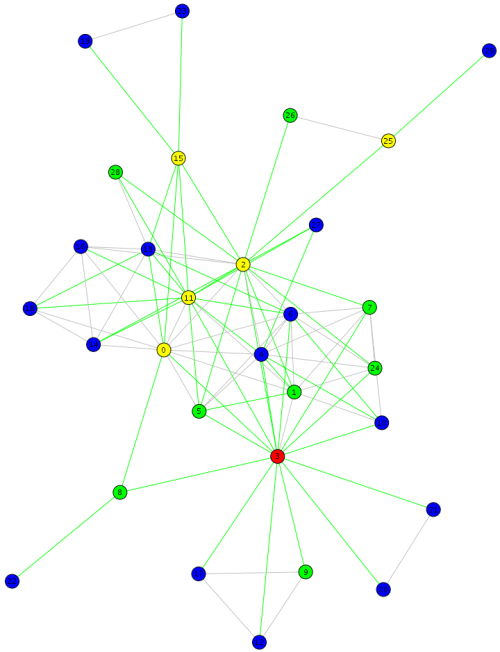
\includegraphics[width=0.4\linewidth]{Chordal.png}
\grph  comes with a bridge to \textsc{GraphStream} which endorses it with
\alert{automatic graph layout and customizable dynamic graph representation}.
\end{frame}


\begin{frame}{Interactive console\demo}
One of the greatest strength of the SageMath Python toolkit is its interactive Python interpreter.
In the same way, \alert{\grph comes with an interactive shell}, by relying on \textsc{BeanShell}.
The interaction language is a dialect of Java.
\begin{flushright}
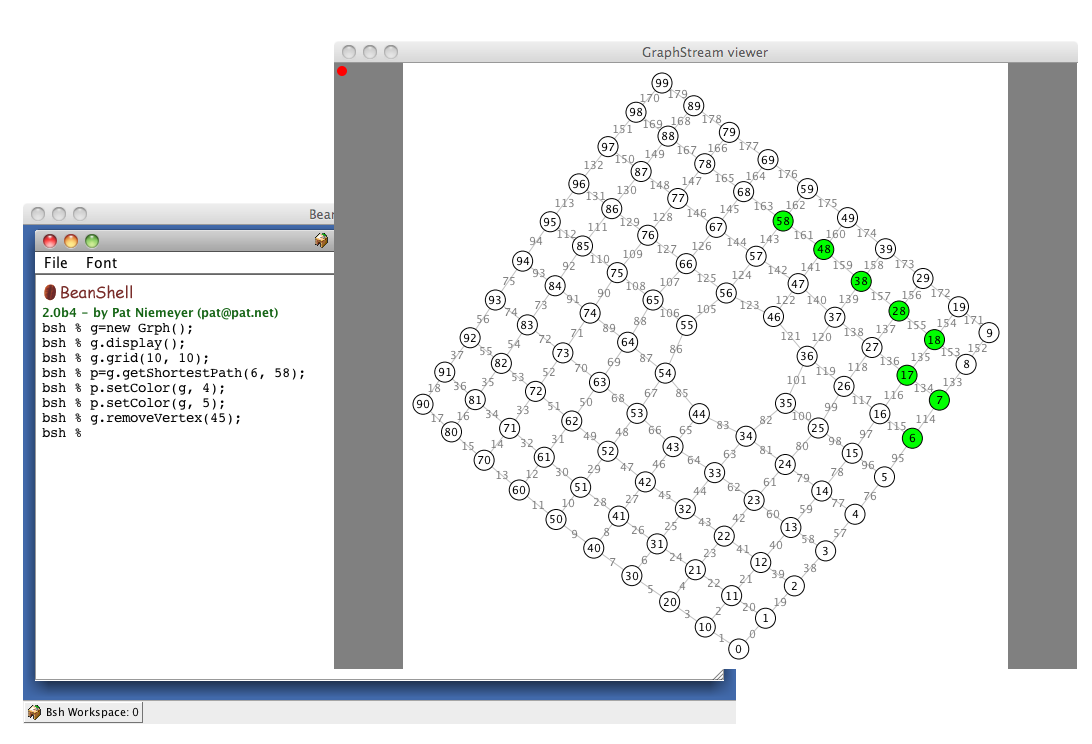
\includegraphics[width=0.7\linewidth]{grph-console.png}
\end{flushright}
\end{frame}


\begin{frame}{Discrete-event engine}
\grph comes with a discrete-event simulation engine that allows it to consider dynamic systems.
	  \begin{itemize}
	    \item mobility models for mobile networks;
	    \item fault models for unreliable networks;
	  \end{itemize}
\end{frame}


\begin{frame}{Experimentation framework\demo}
\grph comes with an experimentation framework that greatly helps the elaboration of usable results by
taking care of:
	  \begin{itemize}
	    \item the non-recomputation of already computed stuff;
	    \item the processing of multi-runs;
	    \item the generation of the plot files.
	  \end{itemize}
	  This greatly simplifies the graph experimentation codes of the user, and scale them down by a large factor.
\end{frame}


\begin{frame}{Framework for evolutionary computing\demo}
\grph comes with a evolutionary computing framework targeted to the
generation of graph instances. This framework, called \textit{Drwin} have the
following particularities:
	  \begin{itemize}
	    \item it does not encode indivdiduals, thereby exploited meaningful
	    application-level operators;
	    \item it is multi-threaded;
	    \item self-adaptive evolution and parallelism;
	    \item OO.
	  \end{itemize}
\end{frame}
		

\begin{frame}{Interoperability\demo}
A \grph graph can be imported/exported as/to:
	  \begin{itemize}
	    \item Grph (compact binary \grph native format);
	    \item GraphText (compct text \grph native format);
	    \item GraphML (XML-dialect);
	    \item GML;
	\item DOT/Graphviz (graph plotter);
	\item DGS (Dynamic Graphs);
	\item Inet/CAIDA Maps  (topology generator);
	  \end{itemize}
	  But also as:
	  \begin{itemize}
	\item JUNG graph;
	\item Mascopt graph;
	  \end{itemize}
\end{frame}


\begin{frame}{Algorithms}
\grph comes with:
\begin{itemize}
\item \alert{basic topology schemes} (grid, ring, chain, star, clique, etc), random schemes (GNP, GNM, random tree), GLP (Generalized Linear Preference), etc.
\item \alert{implementations for common graph algorithms}: 
eccentricity, radius, diameter, in/out vertex/edge degrees, clustering coefficient, density, connected components, minimal spanning tree, shortest paths, BFS/DFS/RS, distributions, maximum clique, minimum vertex cover, maximum independent set, maximum flow, (sub)graph isomorphism, etc.

\end{itemize}
\end{frame}



%\begin{frame}{Think \grph as an abstract framework for YOUR algorithms}
%Since we all have our own definition for metrics (we sometimes don't even agree on what the clustering coefficient is):
%	  \begin{itemize}
%	    \item \grph is best seen as a \alert{framework for the implementation of new algorithms};
%	    \item to this purpose it \alert{provides the basic bricks}: the data structure, the I/O routines, the monitoring tools, the
%	    bridge to C/C++, the parallelism mechanics, etc. 
%	  \end{itemize}
%\alert{The best effort has been made to make it easy the integration of new algorithms.}
%\end{frame}



\section{7 bullets to kill  performance bottlenecks}
\begin{frame}
\sectionti{6 bullets to kill  performance bottlenecks}
\begin{flushright}
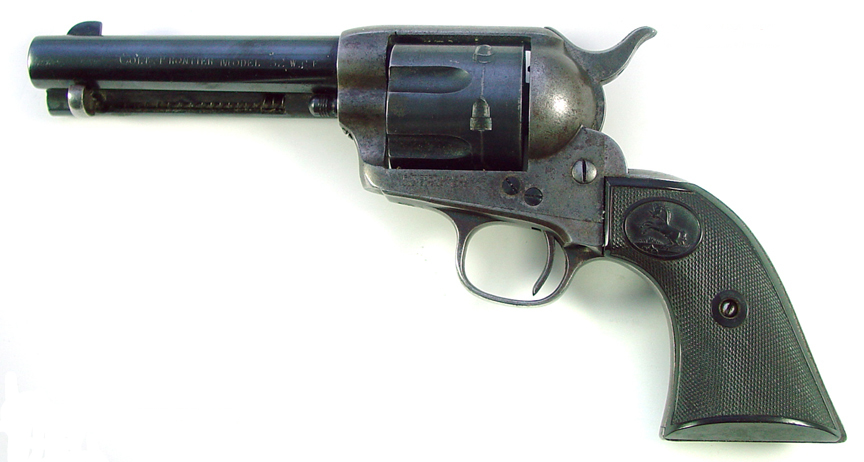
\includegraphics[width=0.5\linewidth]{gun.jpg}
\end{flushright}

\end{frame}

\begin{frame}{Not fully Object Oriented framework}

\alert{Bullet}: In Java, OO kills performance

\begin{itemize}
\item Problem
\item 
	\begin{itemize}
		\item  Java object memory management is too hungry
		\item OO implies an indirection to obtain, anyway, its ID
	 \end{itemize}
\item Solution: \grph considers the vertex (or edge) IS its ID.
\item Advantages:
\item 
	\begin{itemize}
		\item save memory by factor 4
		\item allow much faster management (use of HPPC)
		\item use of low-level caching (speedup 15)
	 \end{itemize}
\end{itemize}
\end{frame}


\begin{frame}{Fast-access incidence lists}

\alert{Bullet}:Both arrays and hash-table are accessed in constant time, but accessing an array is so much faster!
\begin{itemize}
	\item The  implementation of \grph  uses 2 coupled incidence lists.
\end{itemize}
\end{frame}


\begin{frame}{Representing vertex/edge sets as daptative integer sets}

Graph algorithms spend a great deal of their time manipulating vertices and/or edge sets.
\grph proposes three implementations for integer sets:
	  \begin{itemize}
\item based on \alert{hash tables}, adequate when the set is \alert{sparse};
\item based on \alert{bit sets}, adequate when the set is \alert{dense};
\item \alert{adaptative}, adequate when the density evolves unpredicably.
	  \end{itemize}
Bitset-based intsets require at least 32 times less memory than hash-tables-based ones.
When the density cross the threshold 1/32, the implementation of the set is switched.
In order to avoid too frequent implementation switches, \grph uses an hysteresis mechanism.
\end{frame}




\begin{frame}{Caching already computed stuff}
\alert{Bullet 2}: does not compute twice the same thing! \grph makes use of a {\em cache}.
	  \begin{itemize}
\item Basically, \alert{any given property will not be computed twice on the same graph};
this {\em breaks} the complexity of graph operations.
\item For example, the computation of the diameter will return immediately if all-pair shortest paths
were computed previously. This is because diameter requires the distance matrix that was already computed
by the shortest path algorithm.
	  \end{itemize}
Depending on the application, performance  dramatically improves!
\end{frame}



\begin{frame}{Use of C/C++ code}
\alert{Bullet 4}: if you cannot fasten your Java implementation anymore, then write it in C.
\begin{itemize}
\item hackers can expect a speed-up of 5;
\item \grph will find it and \alert{compile it on-the-fly} using optimization flags
for your specific computer;
\item if compilation failed, an optional \alert{100\% pure Java alternative}
will allow the program to run, still.
\end{itemize}
JNI and JNA prove inadequate. Instead Grph resort to process piping. (number of triangles, max-clique, (sub)graph isomorphism, etc)
are already implemented in C++.
\end{frame}


\begin{frame}{Parallelizing algorithms}
\alert{Bullet 5}: take advantage of multi-core computers:
\begin{itemize}
\item algorithms that can be computed independently on every vertex in the graph can be \alert{automatically parallelized};
\item \grph generates a lot more threads that installed cores, hence reducing the probability of unfair load balancing;
\item on my dual-core computer, I experimented \alert{speed-up between 1 and 1.7}.
\end{itemize}
\end{frame}

\begin{frame}{Resorting to linear programming}
\alert{Bullet 6}: benefiting from the advantages of linear programming:
Many graph problems can be expressed as linear programs:
\begin{itemize}
\item the linear program is often shorter than its corresponding algorithm;
\item its resolution benefits from the high efficiency of the solver's strategies for solving.
\end{itemize}
Supported for CPLEX and GLPK (under progress). Invocation of remote solvers (through SSH) is also available. 
\end{frame}


\begin{frame}{Disabling verifications}
\alert{Bullet 7}: a good program is one that checks its parameters. But if you KNOW that the parameters are correct, you can
\alert{disable these time-consuming verifications}.
\begin{itemize}
\item method arguments are checked by assertions;
\item hence they can be disabled;
\item improves ``production'' mode.
\end{itemize}
\end{frame}


\section{Demonstration}
\begin{frame}
\sectionti{Demonstration: let's see how to do things\demo}
	  \begin{itemize}
	    \item creating a graph ($10 \times 10$ grid);
	    \item computing the diameter;
	    \item computing all pair shortest paths;
	    \item adding a new Java algorithm;
	    \item adding a new property to vertices;
	    \item computing a distribution;
	    \item console profiling;
	  \end{itemize}
\end{frame}

\section{Users}
\begin{frame}
\sectionti{Users}
	  \begin{itemize}
	    \item 31 users;
	    \item INRIA, INRA, UCL, Trier, Georgia, Politechnika Warszawska, etc
	  \end{itemize}
\end{frame}


\section{Conclusion}
\begin{frame}
\sectionti{Almost the end}
\end{frame}

\begin{frame}{Conclusion}
	So we have a \alert{graph lib} which design objectives are to maximize:
	  \begin{itemize}
  \item \alert{memory usage} (use of native types);
  \item \alert{computational efficiency} (use of caching, parallelism, etc);
  \item unpronounceability.
  \item \alert{simplicity to use} (simple but functional Java API and tools);
\end{itemize}
\grph is currently used by:
	  \begin{itemize}
  \item Mascotte team at INRIA (at the heart of DRMSim);
%  \item Aoste team at INRIA (in the TimeSquare suite);
  \item You? (no worries, we do provide pro-active support).
\end{itemize}
\end{frame}

\begin{frame}{Conclusion (why would you do so?)}
	I suggest you to take a look at \grph if you want to:
	  \begin{itemize}
  \item to write graph-based scientific applications;
  \item get rid of Java usual inefficiency;
  \item work with me. :)
\end{itemize}
\vfill
\url{http://www-sop.inria.fr/members/Luc.Hogie/grph/}
\end{frame}


\begin{frame}
\begin{center}
\center{\Huge End of the presntation.}

\center{\Huge Any qustions?}

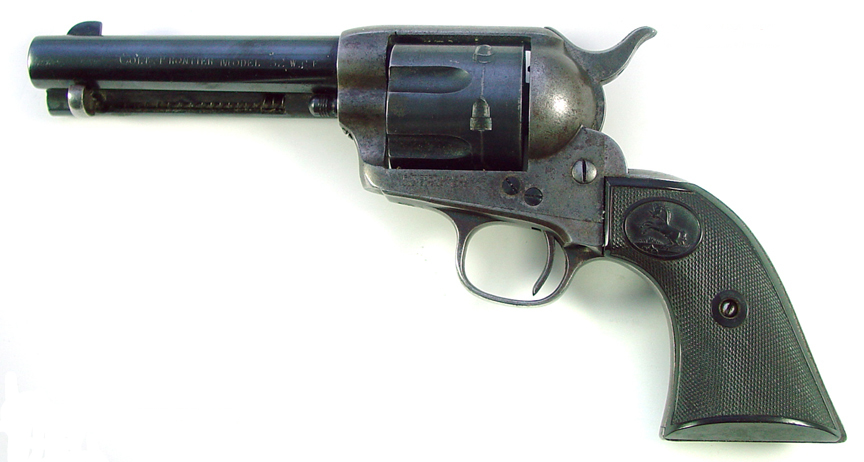
\includegraphics[width=0.4\linewidth]{gun.jpg}
\end{center}
\end{frame}


\end{document}
